\documentclass[11pt,a4paper]{article}
\usepackage{exscale,times}
\usepackage{graphicx}

\usepackage{pgfplots}
\usepackage{amsmath, amssymb, mathtools, contmech}

\setlength{\parindent}{0pt}
\setlength{\parskip}{5pt plus 2pt minus 1 pt}
\topmargin  -5mm
\evensidemargin 8mm
\oddsidemargin  2mm
\textwidth  158mm
\textheight 230mm
\frenchspacing
\sloppy


%%%%%%%%%%%%%%%%%%%%%%%%%%%%%%%%%%%%%%%%%%%%%%%%%%%%%%%%%%%%%%%%%%%%%%%
\begin{document}
\pagestyle{empty}

\begin{center}
%
%   Please insert the title here...
%
{\fontsize{14}{20}\bfseries
FE\textsuperscript{2} for Liquid-Phase Sintering with Seamless Transition from Macroscopic Compressibility to Incompressibility
}
\end{center}

\begin{center}
\textbf{Mikael \"Ohman$^\dagger$$^\ast$, Kenneth Runesson$^\dagger$, Fredrik Larsson$^\dagger$}\\
\bigskip
$^\dagger${Chalmers University of Technology, Department of applied Mechanics}\\
H\"orsalsv\"agen 7a, 41296 G\"oteborg\\ \{mikael.ohman, kenneth.runesson, fredrik larsson\}@chalmers.se\\
\bigskip
\end{center}
%
%   Please insert the keywords here...
%

{\bfseries Keywords}: Liquid phase sintering, Computational homogenization, FE\textsuperscript{2}.

\begin{center}
\textbf{ABSTRACT}\\[1mm]
\end{center}

Powder metallurgy is a versatile technology for the manufacturing of components to (near) net-shape with high product quality. For a hardmetal (such as WC-Co) cold compaction of the powder to a ``green body'' is followed by liquid-phase sintering from the subsequent heating.
This means that the binder metal Co is heated to melt in order to obtain sufficient mobility via capillary action, i.e. via surface traction, stemming from stored surface energy.
Among the early attempts to numerically simulate the surface-tension driven reshaping of contacting particles are those by \cite{JagDaw1988a}.
A recent discussions of surface tension in the context of solid modeling, with extension to anisotropic surface energy, is given in\cite{JavSte2009:2d}.

%
%Please include the abstract here ...
%
In this contribution, liquid phase sintering of particle agglomerates is modeled on the mesoscale as the viscous deformation of particle-particle contact, whereby the single driving force is the surface tension on the particle/pore interface.
On the macroscale, a quasistatic equilibrium problem allows for the prediction of the shrinkage of the sintering body. 
We present a novel FE\textsuperscript{2} formulation of the two-scale sintering problem allowing for the transition to zero porosity, implying macroscale incompressibility.
The seamless transition from compressibility to incompressibility on the macroscale is accomplished by introducing a mixed variational format in terms of (the macroscale) velocity and pressure.
This has consequences also for the formulation of the mesoscale problem, that is complemented with an extra constraint equation.
Hence, the solution fields of the mesoscale problem are the velocity and pressure and, in addition, 
the volumetric part of the macroscopic rate-of-deformation.

% Introduction:
\begin{figure}[thpb!]
  \centering
  %\subfloat[$t = 0$]{
\includegraphics[scale=0.13]{figures/evolve_a}\label{fig:evolve_a}}
  
\includegraphics[scale=0.12]{figures/evolve_a}
  \hspace{1em}
  %\subfloat[$t = 0.45\; t_{\mathrm{end}}$]{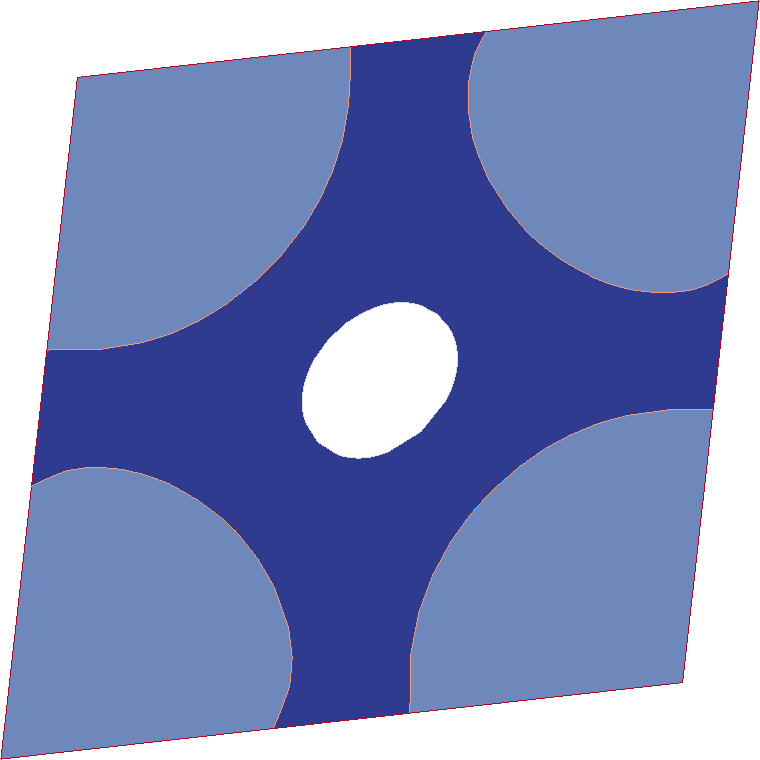
\includegraphics[scale=0.13]{figures/evolve_b}\label{fig:evolve_b}}
  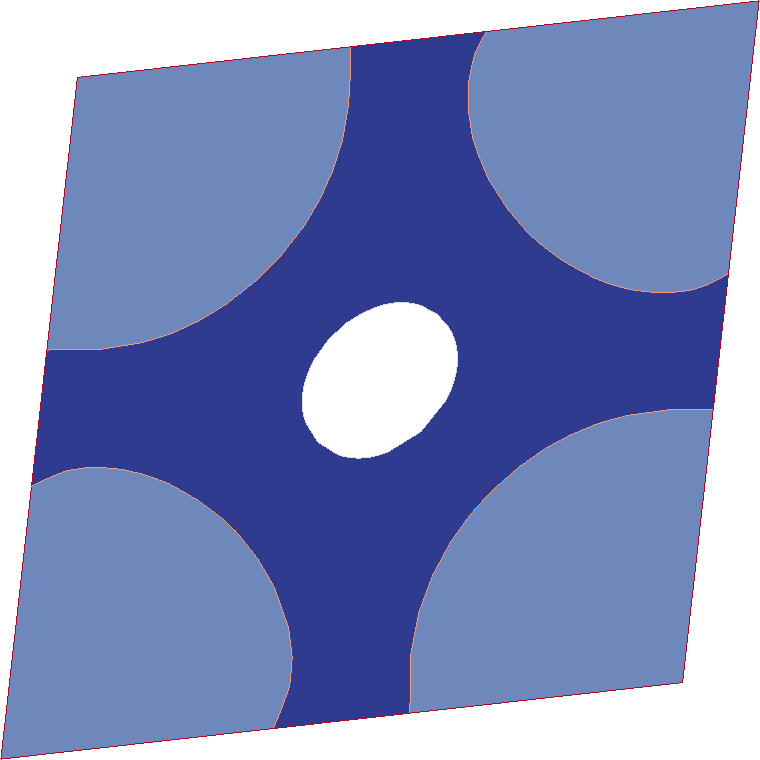
\includegraphics[scale=0.12]{figures/evolve_b}
  \hspace{1em}
  %\subfloat[$t = 0.65\; t_{\mathrm{end}}$]{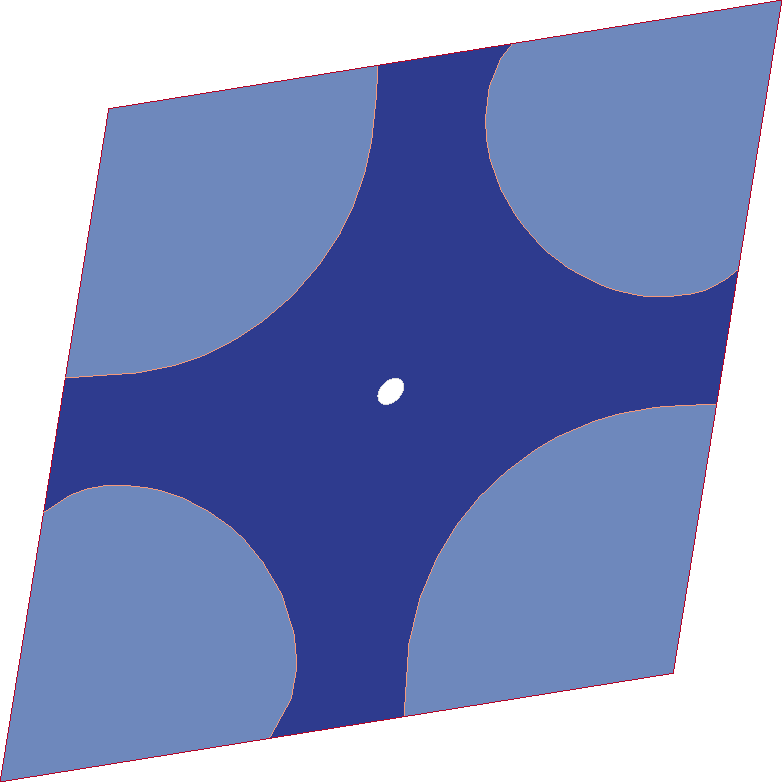
\includegraphics[scale=0.13]{figures/evolve_c}\label{fig:evolve_c}}
  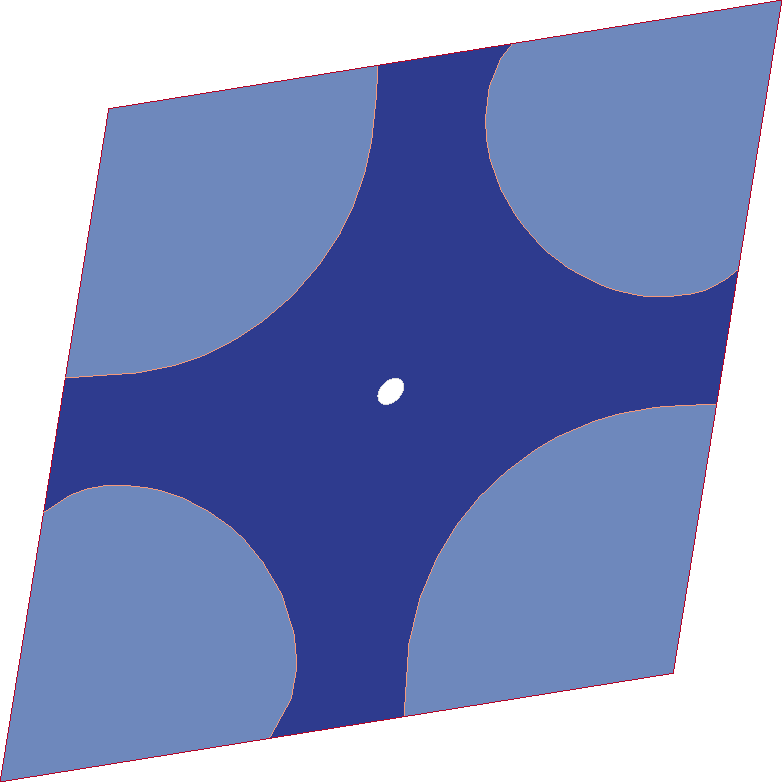
\includegraphics[scale=0.12]{figures/evolve_c}
  \hspace{1em}
  %\subfloat[$t = t_{\mathrm{end}}$]{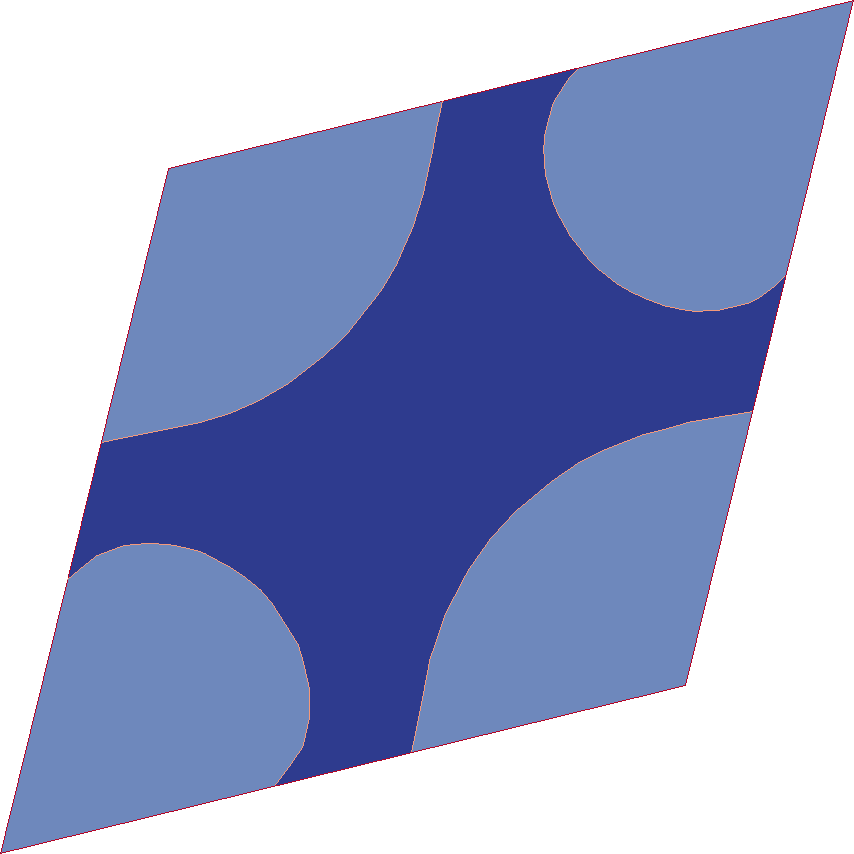
\includegraphics[scale=0.14]{figures/evolve_d}\label{fig:evolve_d}}
  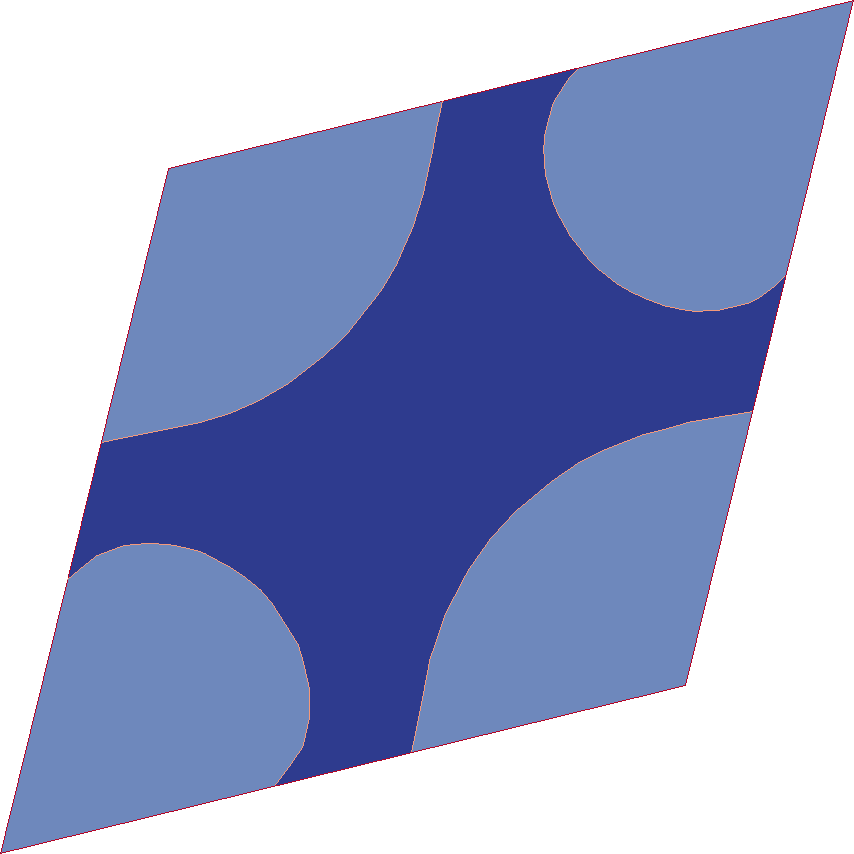
\includegraphics[scale=0.13]{figures/evolve_d}
  \caption{Snapshots of evolving RVE subjected to constant macroscopic shear rate ($\bar{\ts d}_\dev \neq \ts 0$) and zero macroscopic pressure ($\bar{p}=0$).}
  \label{fig:evolve_rve}
\end{figure}
%
\begin{figure}[thpb!]
  \centering
  \begin{tikzpicture}
  \begin{axis}[ yticklabel style={ /pgf/number format/fixed, /pgf/number format/precision=2 },
                tick label style={font=\tiny},font=\footnotesize,
                height=0.2\textheight, width=0.9\textwidth, xmin=0, xmax=1, ymin=-0.5,
                legend style={font=\tiny,at={(1,0)},anchor=south east},
                xlabel={$t_{\mathrm{end}}$}, ylabel={$\bar{d}_\vol$}]
    \addplot[thick,black] table[x=t,y=dvol] {figures/evolve_data_dvol.txt};
  \end{axis}
  \end{tikzpicture}
  \begin{tikzpicture}
  \begin{axis}[ yticklabel style={ /pgf/number format/fixed, /pgf/number format/precision=2 },
                tick label style={font=\tiny},font=\footnotesize,
                height=0.2\textheight, width=0.9\textwidth, xmin=0, xmax=1, ymin=0.83,
                legend style={font=\tiny,at={(1,0)},anchor=south east},
                xlabel={$t_{\mathrm{end}}$}, ylabel={$\rho'$}]
    \addplot[thick,black] table[x=t,y=vof] {figures/evolve_data.txt};
  \end{axis}
  \end{tikzpicture}
  \caption{Evolution of the macroscopic volumetric strain rate ($\bar{d}_\vol$) and relative density ($\rhö́'$) with time for the RVE subjected to constant macroscopic shear rate and zero macroscopic pressure.}
  \label{fig:evolve_graph}
\end{figure}

The numerical example shows the sintering of a single Representative Volume Element (RVE), which is sheared beyond the point where the porosity vanishes while subjected to zero macroscopic pressure.
More specifically, a single unit cell (one pore) is subjected to prescribed macroscopic shear rate, i.e. $\bar{\ts d}_\dev$ takes a constant value ($\bar{\ts d}_\dev$ denotes the deviatoric part of the macroscopic rate-of-deformation tensor), whereas the macroscopic pressure is set to zero, $\bar{p}=0$. This situation of ``mixed control'' represents ``quasi-free'' sintering in the sense that the resulting value of the homogenized subscale stress deviator $\bar{\ts\sigma}_\dev$ is non-zero (while $\bar p = 0 $).
From the computations, it turns out that $\bar{\ts\sigma}_\dev$ stays nearly constant throughout the entire simulation time.
Snapshots of the evolving RVE-configuration are given in Figure \ref{fig:evolve_rve}, and it appears that effects of the adopted Dirichlet boundary condition on the RVE are clearly visible in the severely sheared state.
The evolution of $\bar d_\vol$, which is a primary variable in the RVE-problem, and of the macroscopic relative density, $\rho'$, is shown in Figure \ref{fig:evolve_graph}.
Vanishing porosity, i.e. macroscopic incompressibility manifested by $\bar d_\vol = 0$ and $\rho' = 1$, was reached at around $0.69\;t_{\mathrm{end}}$.
After this point in time, the deformation continues, but it is completely isochoric.

\begin{thebibliography}{99}
\bibitem{JagDaw1988a} A.~Jagota, P.~R.~Dawson: Micromechanical modeling of powder compacts --- I. Unit problems for sintering and traction induced deformation. \textit{Acta Metallurgica}, 36 (1988), 2551--2561. 
\bibitem{JavSte2009:2d} A.~Javili, P.~Steinmann: A finite element framework for continua with boundary energies. Part I: The two-dimensional case. \textit{Computer Methods in Applied Mechanics and Engineering}, 198 (2009), 2198--2208.
%\bibitem{Stein} E. Stein, M. Rueter, S. Ohnimus: Adaptive finite element analysis and modelling of solids and structures. Findings, problems and trends. \textit{International Journal for Numerical Methods in Engineering}, 60 (2004), 103--138. 
\end{thebibliography}

\end{document}
